\documentclass[a0poster,colspace=15pt,innermargin=15pt,blockverticalspace=15pt]{tikzposter} % See Section 3
\title{Experimenting with the Gram-Schmidt Walk\vspace{-2ex}} \institute{Chair of Combinatorial Analysis} % See Section 4.1
\author{Gaëtan Bossy\\
Supervision by Pr. Adam Marcus} %\titlegraphic{\includegraphics[height=2cm]{logo-epfl-rogned.png}}
\usetheme{Envelope} % See Section 5
\usepackage[linesnumbered,ruled,vlined]{algorithm2e}%ruled in 1st param

%to fix algo issues
\AtBeginEnvironment{algorithm}{%
  \setlength{\columnwidth}{\linewidth}%
}

%to include pdf plots
\usepackage{pdfpages}

%To do loops
\usepackage{multido}

%to include plots generated in python
\usepackage[utf8]{inputenc}
\usepackage{pgfplots}
\DeclareUnicodeCharacter{2212}{−}
\usepgfplotslibrary{groupplots,dateplot}
\usetikzlibrary{patterns,shapes.arrows}
\pgfplotsset{compat=newest}


\definetitlestyle{sampletitle}{
width=500mm, roundedcorners=20, linewidth=2pt, innersep=5pt,
titletotopverticalspace=0mm, titletoblockverticalspace=0mm,titlegraphicheight=0mm
}{
\begin{scope}[line width=\titlelinewidth, rounded corners=\titleroundedcorners]
\draw[color=blocktitlebgcolor, fill=titlebgcolor]
(\titleposleft,\titleposbottom) rectangle (\titleposright,\titlepostop);
\end{scope}
}

\usetitlestyle{Envelope}%Default, Basic, Envelope, Wave, VerticalShading,Filled, Empty
%Wave too big

%to bold symbols
\usepackage{bm}

\usepackage{amsmath}
%\usepackage{amsthm}
\usepackage{amssymb}
\DeclareMathOperator{\Span}{span}
\newtheorem{theorem}{Theorem}

\begin{document}

\maketitle[titletotopverticalspace=0pt,titletoblockverticalspace=15pt,innersep=0pt] % See Section 4.1
\begin{columns} % See Section 4.4
\column{0.6}
\begin{subcolumns}
\subcolumn{0.8}
\block[%bodywidthscale=0.83,titlewidthscale=0.83,bodyoffsetx=-4cm,
bodyinnersep=0.4cm]{Banaszczyk's Theorem}{
A fondamental theorem in discrepancy theory is the following result:
\begin{theorem}[Banaszczyk, 1998]\label{banaszczyk}
For all convex body $K \subseteq \mathbb{R}^d$, with Gaussian measure $\gamma_m(K)\geq 1/2$, and given $\textbf{v}_1, \dots, \textbf{v}_n \in \mathbb{R}^d$, $\|\textbf{v}_i\|_2 \leq 1$ for all $i$, then there exists $ \textbf{z} \in \{-1, 1\}^n$ such that
$\sum_{i=1}^n \textbf{z}(i)\textbf{v}_i \in 5K. $
\end{theorem}
%The Gaussian measure of a body is defined as $\gamma_m(S) = \mathbb{P}[\textbf{g} \in S] = \int_{\textbf{y} \in S} \frac{1}{(2 \pi)^{m/2}} e^{-||\textbf{y}||^2/2} d\textbf{y}$ where $\textbf{g}$ is a standard Gaussian random vector in $\mathbb{R}^m$, i.e. $\textbf{g} \sim \mathcal{N}(0, I_m)$. 

While this results gives the best known bounds for several well-known discrepancy problems, its proof is non-constructive. For years, mathematicians tried to come up with a constructive algorithm to generate the colorings whose existence is proved by the theorem. In 2016, Dadush, Garg, Lovett and Nikolov proved that actually, all that is needed is an algorithm to generate a coloring $\textbf{z}$ such that the corresponding \textbf{vector of imbalances}, $\textbf{Bz}$, where $\textbf{B}= (\textbf{v}_1, \dots, \textbf{v}_n) \in \mathbb{R}^{d \times n}$, would be $\sigma$-subgaussian with $\sigma>0$ a constant.

%A random vector $\textbf{Y} \in \mathbb{R}^m$ is said to be subgaussian with parameter $\sigma$ (or $\sigma$-subgaussian) if for all $\bm{\theta} \in \mathbb{R}^m$:$\mathbb{E}\left[e^{\langle\textbf{Y},\bm{\theta}\rangle}\right]\leq e^{\sigma^2\|\bm{\theta}\|_2^2/2}.$
%A $\sigma$-subgaussian vector is basically at least as centered as a gaussian vector with the same variance $\sigma^2$.

}
%\note[width=18cm,connection,targetoffsetx=23cm,targetoffsety=5cm]{The Gaussian measure of a body is defined as $%$
%\gamma_m(S) = \mathbb{P}[\textbf{g} \in S]% = \int_{\textbf{y} \in S} \frac{1}{(2 \pi)^{m/2}} e^{-||\textbf{y}||^2/2} d\textbf{y}$
%$ where $\textbf{g}$ is a standard Gaussian random vector in $\mathbb{R}^m$, i.e. $\textbf{g} \sim \mathcal{N}(0, I_m)$.}
\subcolumn{0.2}
\note[width=9.8cm,targetoffsetx=17.1cm,targetoffsety=6.1cm,innersep=0.4cm]{The Gaussian measure of a body is defined as $$
\gamma_m(S) = \mathbb{P}[\textbf{g} \in S]% = \int_{\textbf{y} \in S} \frac{1}{(2 \pi)^{m/2}} e^{-||\textbf{y}||^2/2} d\textbf{y}
$$ where $\textbf{g}$ is a standard Gaussian random vector in $\mathbb{R}^m$, i.e. $\textbf{g} \sim \mathcal{N}(0, I_m)$.}

%\note[width=13cm,targetoffsetx=18cm,targetoffsety=5cm,innersep=0.4cm]{The Gaussian measure of a body is defined as $$\gamma_m(S) = \int_{\textbf{y} \in S} \frac{1}{(2 \pi)^{m/2}} e^{-||\textbf{y}||^2/2} d\textbf{y}.$$}

\note[width=9.8cm,targetoffsetx=17.1cm,targetoffsety=-2.5cm,innersep=0.4cm]{A random vector $\textbf{Y} \in \mathbb{R}^m$ is said to be subgaussian with parameter $\sigma$ (or $\sigma$-subgaussian) if for all $\bm{\theta} \in \mathbb{R}^m$:$$\mathbb{E}\left[e^{\langle\textbf{Y},\bm{\theta}\rangle}\right]\leq e^{\sigma^2\|\bm{\theta}\|_2^2/2}.$$}

\end{subcolumns}

\block[bodyinnersep=0.4cm]{The Gram-Schmidt Walk Algorithm}{
%\section{General idea}
%The idea of the algorithm is that it walks step by step in the hypercube of dimension $n$, $[-1,1]^n$. We start at some initial fractional coloring $\textbf{z}_0\in[-1,1]^n$. At each step, the coloring moves in the hypercube until at least one additional coordinate becomes 1 or -1, that is it moves to a facet of the hypercube it wasn't on yet. Once a coordinate is set to -1 or 1, it won't move for the rest of the algorithm, thus after step $i$ our fractional coloring is in the intersection of at least $i$ different facets. From all this, we can see that the algorithm reaches a non fractional coloring $\textbf{z}_t\in\{-1,1\}^n$ in at most $n$ steps.

%The question now becomes "how to choose the facet to move to ?". To do so, the algorithm finds an update direction $\textbf{u}_t\in\mathbb{R}^n$ such that $\sum_{i=1}^n\textbf{u}_t(i)\textbf{v}_i$ is small, and updates $\textbf{z}_t$ into $\textbf{z}_{t+1}=\textbf{z}_t+\delta_t\textbf{u}_t$. $\delta_t\in\mathbb{R}$ is chosen so that $\textbf{z}_{t+1}\in[-1,1]^n$ and at least one additional coordinate now has absolute value 1. Moreover, $\delta_t$ is chosen randomly among the two potential candidates that fulfill the previously mentioned condition, and the distribution between the two candidates is engineered so that its expectation is 0 and no direction is favored. Thus before the algorithm starts, ending at $\textbf{z}_t\in\{-1,1\}^n$ or at $-\textbf{z}_t\in\{-1,1\}^n$ is equally likely.

%\section{Pseudocode}
%The algorithm takes as input $\textbf{v}_1,\ldots,\textbf{v}_n\in\mathbb{R}^d$, and an initial coloring $\textbf{z}_0\in[-1,1]^n$. A run of the algorithm consists of at most $n$ time steps because at least an element is colored during each step thanks to the choice of $\delta_t$. At the end of each time step $t$, the algorithm obtains a fractional coloring $\textbf{z}_t\in[-1,1]^n$. An element $i \in [n]$ is said to be \textit{alive} at time $t$ if $|\textbf{z}_{t-1}(i)|<1$, and \textit{fixed} otherwise. Let $A_t=\{i\in[n]:|\textbf{z}_{t-1}(i)|<1\}$. The \textit{pivot} $p(t)$ is an element that is alive at time $t$, which can for example be chosen as the largest indexed element among the elements that are still alive. We define the set $V_t$ as $\Span\{\textbf{v}_i:i\in A_t,i\not=p(t)\}$. We denote by $\Pi_{V_t^\perp}$ the projection operator on $V_t^\perp$. Finally, we need $\textbf{v}^{\perp}(t)=\Pi_{V_t^\perp}(\textbf{v}_{p(t)})$ as the projection of the pivot vector over all alive vectors. 
\begin{algorithm}[H]\label{walk}
{\fontsize{32}{32}
\caption{\textbf{The Gram-Schmidt Walk} (\textbf{GSW})
%, a vector balancing algorithm 
by Dadush, Bansal, Garg and Lovett, 2018}
    \SetKwInOut{Input}{Input}
    \SetKwInOut{Output}{Output}
    \Input{$\textbf{v}_1,\ldots,\textbf{v}_n\in\mathbb{R}^d$%with $\ell_2$ norm  at most 1
, an initial coloring $\textbf{z}_0\in[-1,1]^n$}
    \Output{a coloring $\textbf{z}_n \in \{-1,1\}^n$}
   $t=1$, $A_1=\{i\in[n]:|\textbf{z}_0(i)|<1\}$ and $p(1) = \max \{i \in A_1\}$\\
    \While{$A_t\not=\emptyset$}{
       % Compute $\textbf{u}_t\in\mathbb{R}^n$ such that
%        $\begin{cases}
%            \textbf{u}_t(p(t)) =1\\
%            \textbf{u}_t(i) =0 \text{ if } i \notin A_t\\
%            \textbf{v}^\perp(t) = \textbf{v}_{p(t)} + \sum_{i \in A_t\setminus\{p(t)\}} \textbf{u}_t(i)\textbf{v}_i\\
%        \end{cases}$\\
$\textbf{u}_t = \arg\min_{\textbf{u} \in U} \|\textbf{Bu}\|$ where $U=\{u\in\mathbb{R}^n:u(p(t))=1$ and $u(i)=0\forall i\not\in A_t\}$\\
        $\Delta = \{\delta : \textbf{z}_{t-1} + \delta \textbf{u}_t \in [-1,1]^n\}$, let $\begin{cases}
            \delta_t^+ = \max \Delta\\
            \delta_t^- = \min \Delta
        \end{cases}$then $\delta_t = \begin{cases}
            \delta_t^+ \text{ w.p. } \frac{-\delta_t^-}{(\delta_t^+ - \delta_t^-)}\\
            \delta_t^- \text{ w.p. } \frac{\delta_t^+}{(\delta_t^+ - \delta_t^-)}
        \end{cases}$\\
        $\textbf{z}_t = \textbf{z}_{t-1} + \delta_t \textbf{u}_t$, $t\leftarrow t+1$,  $A_t=\{i\in[n]:|\textbf{z}_{t-1}(i)|<1\}$, $p(t) = \max \{i \in A_t\}$
    }
    Output $\textbf{z}_T\in\{-1,1\}^n$.
    %\caption{Gram-Schmidt walk}
    }%
    \end{algorithm}
 When $\textbf{z}_0=\textbf{0}$, this algorithm produces an assignment $\textbf{z}$ such that the corresponding vector of imbalances, $\textbf{Bz}$, has a small norm. One small modification one can do is to always choose the $\delta$ with the smallest absolute value in line 4. We call this modification the \textbf{Deterministic Gram-Schmidt Walk} (\textbf{DGSW}). Note that it is still random thanks to the choice of the pivot.

A basic implementation of this algorithm takes time $O(n^3d)$ to run, but as can be seen in my thesis, a smart implementation can speed that up to $O(n^2d)$. Using brute force to choose the assignment with the shortest vector of imbalances is inneficient as it takes time $O(2^nd)$, we name that variant \textbf{Lowest Norm Assignment} (\textbf{LNA}).

The following result shows that this algorithm can be used to sample colorings from theorem \ref{banaszczyk}.
\begin{theorem}[Harshaw, Spielman, Zhang, Sävje, 2019]
    For $\textbf{z}$ sampled via the Gram-Schmidt walk with input $\textbf{v}_1, \dots, \textbf{v}_n\in \mathbb{R}^{d}$ with euclidean norm at most 1, we have that $\textbf{Bz}$ is subgaussian with parameter $\sigma^2=1$.%:$$\mathbb{E}[exp(\langle\textbf{Bz},\textbf{v}\rangle)]\leq exp(\|\textbf{v}\|^2_2/2)\quad\forall\textbf{v}\in\mathbb{R}^{n+d}$$
\end{theorem}
} 



%\note[width=2cm,targetoffsetx=14.7cm,targetoffsety=0.5cm,innersep=0.4cm,connection,radius=8cm, angle=80]{}
\colorlet{notefrcolor}{green} 
\colorlet{notebgcolor}{green} 
\note[width=12cm,targetoffsetx=11.4cm,targetoffsety=4.2cm,innersep=0.4cm,connection,angle=-15,radius=8cm]{$(\textbf{z}_t)_{t\in\{1,\dots,n\}}$ is actually a martingale as $\mathbb{E}[\delta_t|\delta_t^+,\delta_t^-]=0$.}

\note[width=13cm,targetoffsetx=10.5cm,targetoffsety=7.1cm,innersep=0.4cm,connection, angle=0, radius=12cm]{If $V_t=\Span\{\textbf{v}_i:i\in A_t\setminus\{p(t)\}\}$, $\textbf{u}_t$ can be chosen as a solution of $\Pi_{V_t}(\textbf{v}_{p(t)}) + \sum_{i \in A_t\setminus\{p(t)\}} \textbf{u}_t(i)\textbf{v}_i=\textbf{0}$, $\textbf{u}_t\in U$ where $\Pi_{V_t}$ is the projector on $V_t$.}

\note[width=13cm,targetoffsetx=1cm,targetoffsety=9.8cm,innersep=0.4cm,connection,radius=8cm, angle=4]{Here and at the end of line 5, this is equivalent to choosing the pivot randomly out of $A_t$ when the previous pivot has been colored.}

%\note[width=12cm,targetoffsetx=11.5cm,targetoffsety=-2cm,innersep=0.4cm]{}

%\note[width=13cm,targetoffsetx=18cm,targetoffsety=5cm,innersep=0.4cm]{The Gaussian measure of a body is defined as $$\gamma_m(S) = \int_{\textbf{y} \in S} \frac{1}{(2 \pi)^{m/2}} e^{-||\textbf{y}||^2/2} d\textbf{y}.$$}

%\note[width=10cm,targetoffsetx=17cm,targetoffsety=-3.5cm,innersep=0.4cm]{A random vector $\textbf{Y} \in \mathbb{R}^m$ is said to be subgaussian with parameter $\sigma$ (or $\sigma$-subgaussian) if for all $\bm{\theta} \in \mathbb{R}^m$:$$\mathbb{E}\left[e^{\langle\textbf{Y},\bm{\theta}\rangle}\right]\leq e^{\sigma^2\|\bm{\theta}\|_2^2/2}.$$}


\block[bodyinnersep=0.4cm]{Changing the Pivot Rule}{
In the pseudocode given above, the pivot $p(t)$ is chosen through the order of the input vector. It could also be chosen randomly, as that would be equivalent to shuffling the input vectors which do not have a specific order. One area of potential improvement for this algorithm is to add rules for the choice of the pivot. For example, it could depend on the norm of the vectors in $A_t$, on  how much they would move the vector of imbalances in expectation, or on the fractional coloring. 

One promising variant that seems to improve the algorithm regarding the minimization of the vector of imbalances is to choose the pivot as $p(t)=\arg\max_{i\in A_t}|x(i)|$. This rule, that we call \textbf{maximum absolute coloring} (\textbf{MAC}), changes the behavior of the algorithm as can be seen in figure \ref{max_col_comp}, which shows vector of imbalances produced from 100 runs of several variant of the GSW with 100 vectors sampled uniformly from the ball of radius 1 as input, and figure \ref{max_col_norms} which shows the average norm of several variants of the GSW across various number of input vectors $n$ and dimension $d$. The assignments produced using this rule result in notably shorter vector of imbalances, especially when coupled with the DGSW. In my thesis, we explore several potential modifications of the algorithm including this one.
}

\block[bodyinnersep=0.4cm]{GSW Variants Comparison}{
\begin{tikzfigure}[Plot of average norm of vectors of imbalances for the GSW, the GSW with MAC and the DGSW with MAC, each obtained from an input of $n$ vectors sampled uniformly from the ball of radius 1 in $\mathbb{R}^d$ with random pivot rule and maximum absolute coloring pivot rule. For small $n$'s, we also show the norm of the LNA. Results are averaged over 1000 runs except for the LNA with $n=20$ where they're averaged over 20 runs as the running time is too long to do more of them.\par\vspace{-1ex}]
\vspace{-1ex}\hspace{-3ex}
% This file was created with tikzplotlib v0.10.1.
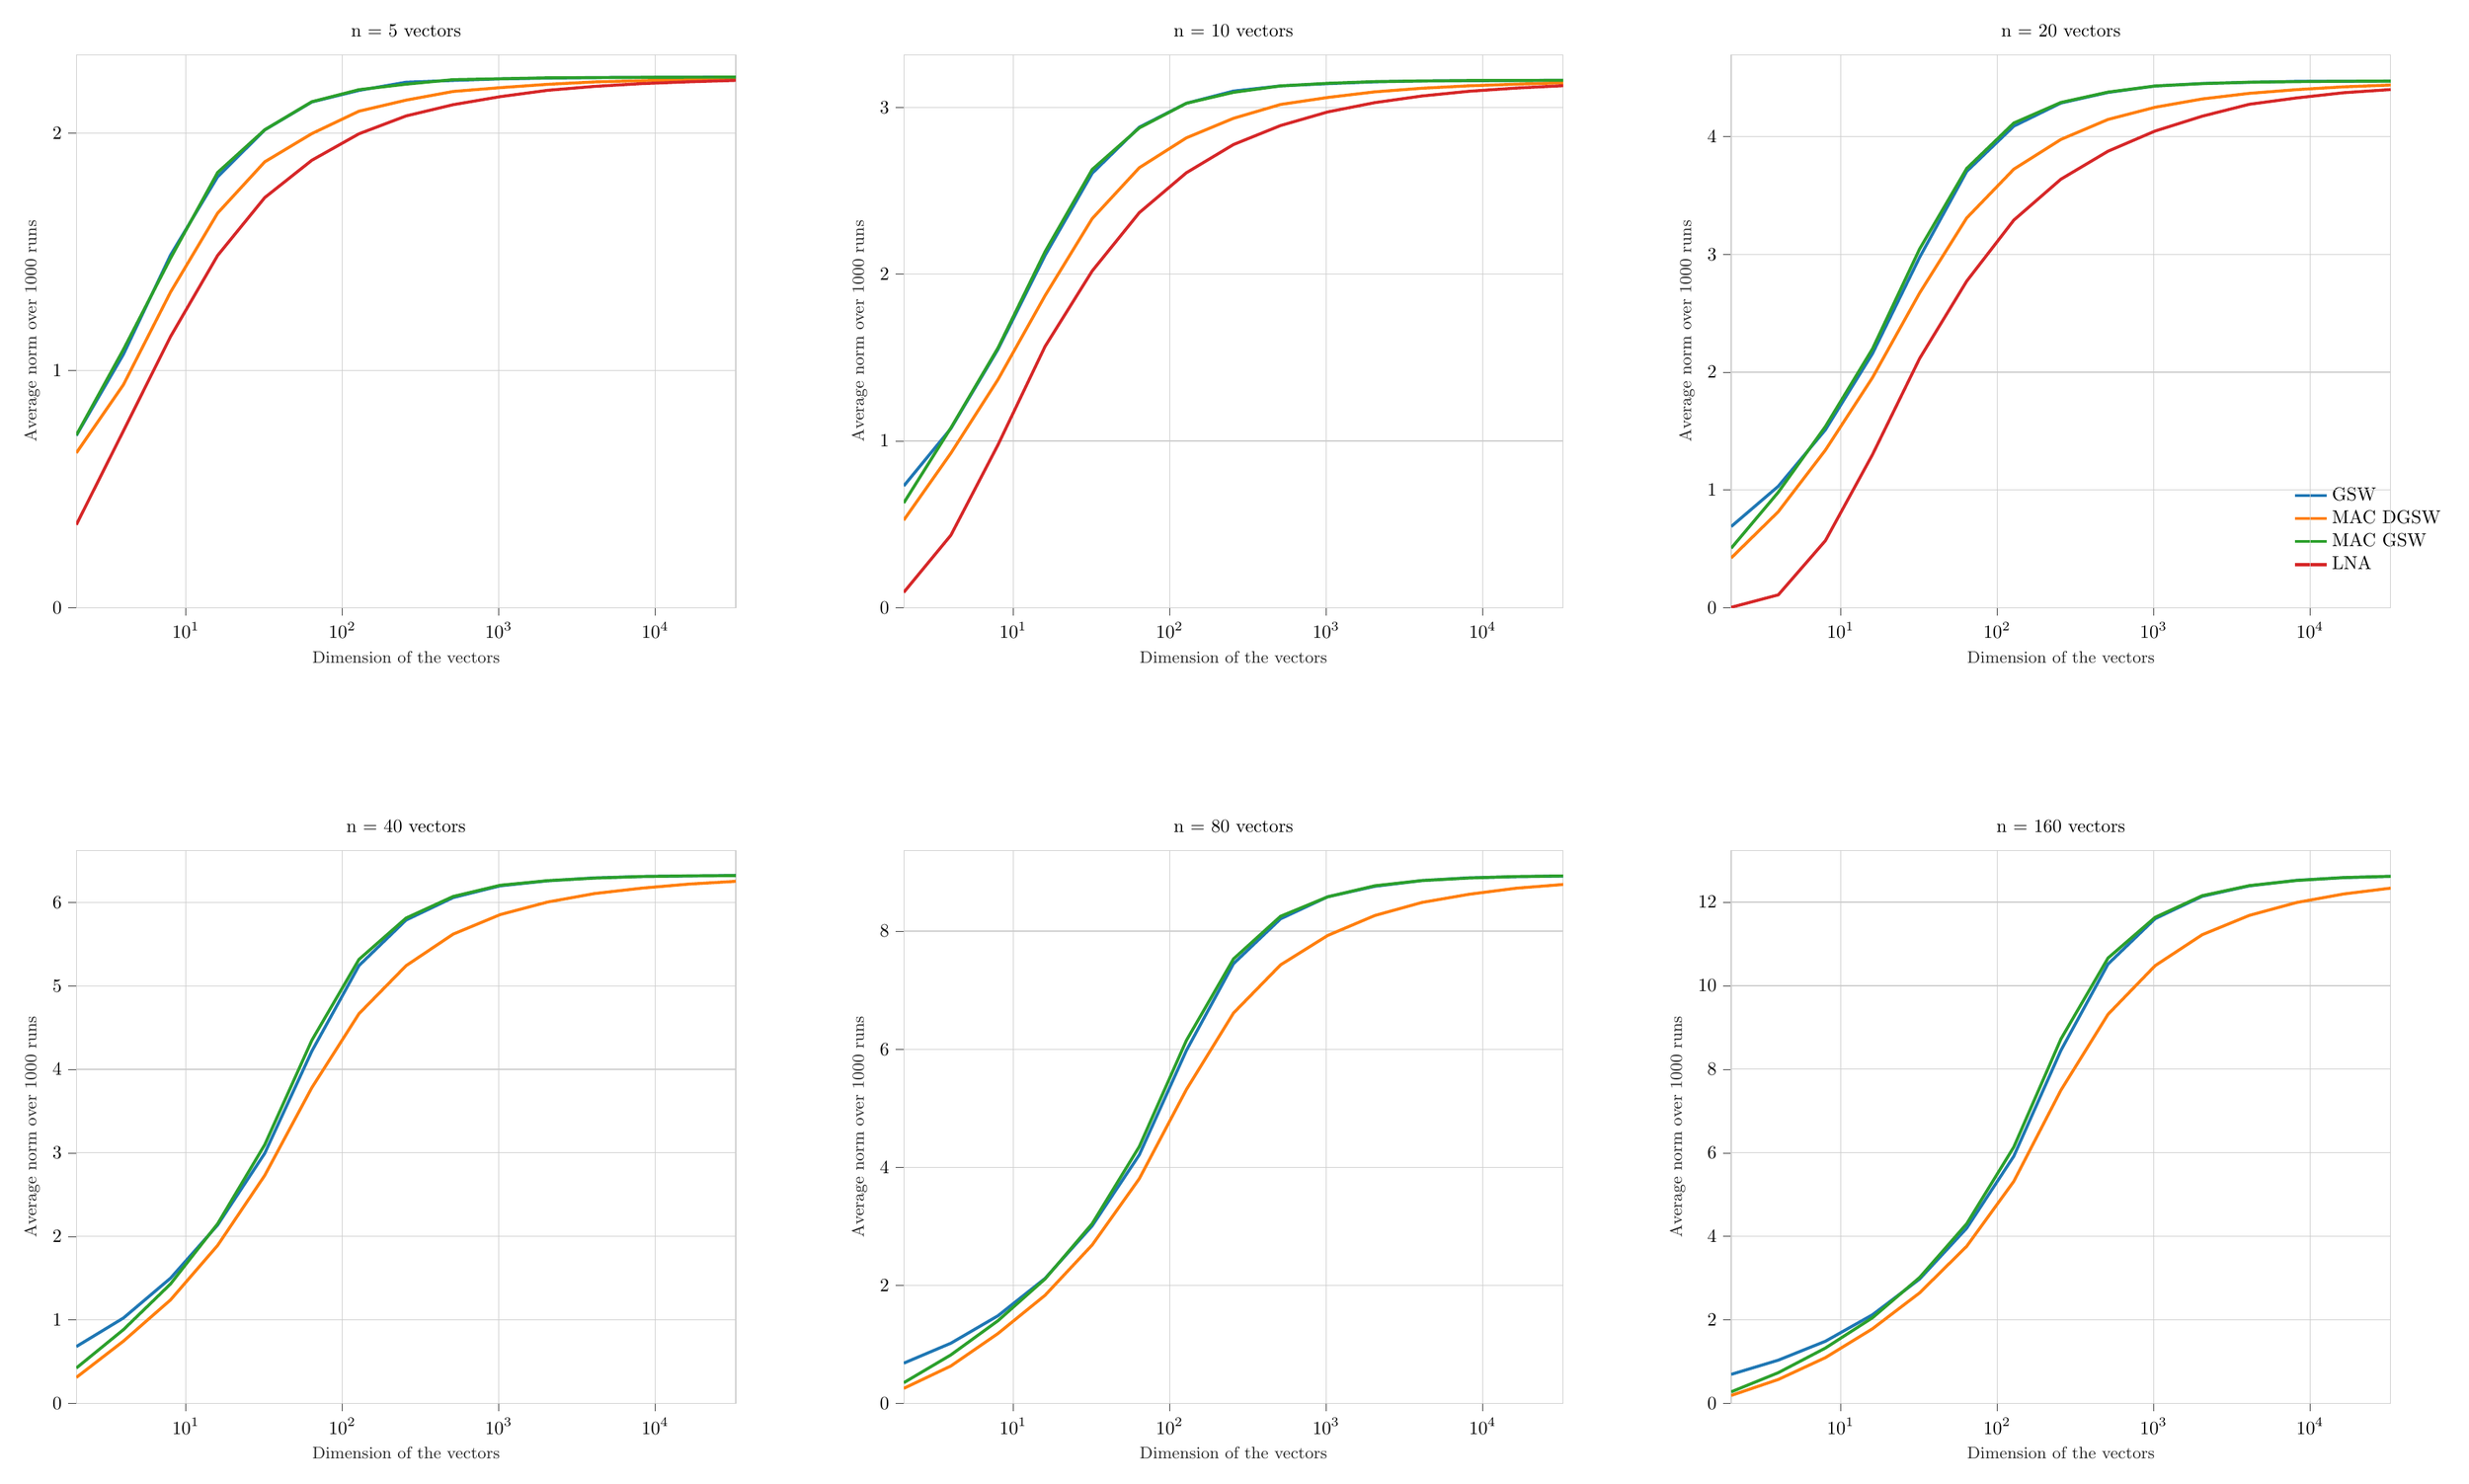
\begin{tikzpicture}

\definecolor{crimson2143940}{RGB}{214,39,40}
\definecolor{darkorange25512714}{RGB}{255,127,14}
\definecolor{darkslategray38}{RGB}{38,38,38}
\definecolor{forestgreen4416044}{RGB}{44,160,44}
\definecolor{lightgray204}{RGB}{204,204,204}
\definecolor{steelblue31119180}{RGB}{31,119,180}

\begin{groupplot}[group style={group size=3 by 2, vertical sep=130pt, horizontal sep=90 pt,ylabels at=edge left},width=14cm,height=12cm,xmin=2, xmax=32768]
\nextgroupplot[
axis line style={lightgray204},
legend cell align={left},
legend style={
  fill opacity=0.8,
  draw opacity=1,
  text opacity=1,
  at={(3.6,0.05)},
  anchor=south east,
  draw=none
},
log basis x={10},
ytick distance=0.5,
tick align=outside,
tick pos=left,
title={n = 5 vectors},
x grid style={lightgray204},
xlabel=\textcolor{darkslategray38}{\small Dimension of the vectors},
xmajorgrids,
xmode=log,
xtick style={color=darkslategray38},
xtick={0.1,1,10,100,1000,10000,100000,1000000},
xticklabels={
  \(\displaystyle 10^{-1}\),
  \(\displaystyle 10^{0}\),
  \(\displaystyle 10^{1}\),
  \(\displaystyle 10^{2}\),
  \(\displaystyle 10^{3}\),
  \(\displaystyle 10^{4}\),
  \(\displaystyle 10^{5}\),
  \(\displaystyle 10^{6}\)
},
y grid style={lightgray204},
ylabel=\textcolor{darkslategray38}{\small \small Average norm over 1000 runs},
ymajorgrids,
ymin=0, ymax=2.33037203007402,
ytick style={color=darkslategray38},
ytick={0,1,2},
yticklabels={
  \(\displaystyle 0\),
  \(\displaystyle 1\),
  \(\displaystyle 2\),
}
]
\addplot [ultra thick, steelblue31119180]
table {%
2 0.725885247935057
4 1.06804241875013
8 1.48630027825432
16 1.81589859843917
32 2.01346123112685
64 2.13110037485254
128 2.1797687419633
256 2.21448764797278
512 2.22182715791898
1024 2.22846121023495
2048 2.2315937632598
4096 2.23395401718205
8192 2.23471819471962
16384 2.23541268109728
32768 2.23606837435418
};
\addlegendentry{GSW}
\addplot [ultra thick, darkorange25512714]
table {%
2 0.652410710514138
4 0.93998864267492
8 1.33006272444076
16 1.66304253507335
32 1.87891007238734
64 1.99779701950075
128 2.09225031565771
256 2.13884143681023
512 2.1754057939251
1024 2.19144836589604
2048 2.20537735152823
4096 2.21557801446247
8192 2.22073140842868
16384 2.225816873593
32768 2.22928673619057
};
\addlegendentry{MAC DGSW}
\addplot [ultra thick, forestgreen4416044]
table {%
2 0.727627960594836
4 1.08845812674368
8 1.4727280779802
16 1.8340289357929
32 2.01401182855433
64 2.13221027341244
128 2.18296020044521
256 2.2060792686017
512 2.22525503977098
1024 2.22902136469112
2048 2.23297397933754
4096 2.2338152894887
8192 2.23492015930732
16384 2.23546501095428
32768 2.23573994455621
};
\addlegendentry{MAC GSW}
\addplot [ultra thick, crimson2143940]
table {%
2 0.349995259957233
4 0.745586905456825
8 1.14261938161702
16 1.48448275215293
32 1.72829394412234
64 1.88554075674287
128 1.99697706538675
256 2.07223793651122
512 2.1197049607246
1024 2.15357196582785
2048 2.18013050882434
4096 2.19675426428705
8192 2.20842349777013
16384 2.21612086336389
32768 2.2221087026373
};
\addlegendentry{LNA}

\nextgroupplot[
axis line style={lightgray204},
log basis x={10},
tick align=outside,
tick pos=left,
title={n = 10 vectors},
x grid style={lightgray204},
xlabel=\textcolor{darkslategray38}{\small Dimension of the vectors},
xmajorgrids,
xmode=log,
xtick style={color=darkslategray38},
xtick={0.1,1,10,100,1000,10000,100000,1000000},
xticklabels={
  \(\displaystyle 10^{-1}\),
  \(\displaystyle 10^{0}\),
  \(\displaystyle 10^{1}\),
  \(\displaystyle 10^{2}\),
  \(\displaystyle 10^{3}\),
  \(\displaystyle 10^{4}\),
  \(\displaystyle 10^{5}\),
  \(\displaystyle 10^{6}\)
},
y grid style={lightgray204},
ylabel=\textcolor{darkslategray38}{\small Average norm over 1000 runs},
ymajorgrids,
ymin=0, ymax=3.3153130011071,
ytick style={color=darkslategray38},
ytick={0,1,2,3},
yticklabels={
  \(\displaystyle 0\),
  \(\displaystyle 1\),
  \(\displaystyle 2\),
  \(\displaystyle 3\),
}
]
\addplot [ultra thick, steelblue31119180]
table {%
2 0.730387977140844
4 1.07454562271808
8 1.54905923158289
16 2.11200756982195
32 2.60415146745229
64 2.88077355026236
128 3.02414941788804
256 3.09728598016533
512 3.12830632964603
1024 3.14161978031348
2048 3.15254200838075
4096 3.15799663218289
8192 3.15920166939847
16384 3.16111714253532
32768 3.16152483513855
};
\addplot [ultra thick, darkorange25512714]
table {%
2 0.525336091041823
4 0.926648372109926
8 1.36795988842879
16 1.8711573310637
32 2.33258856840569
64 2.6375997786384
128 2.81675747971372
256 2.93388976773843
512 3.01694392077739
1024 3.05886625454876
2048 3.09249162798751
4096 3.1141177437442
8192 3.12863323068566
16384 3.13851859153112
32768 3.14659991948233
};
\addplot [ultra thick, forestgreen4416044]
table {%
2 0.628522904871021
4 1.07822237844356
8 1.5576477768795
16 2.13496982295936
32 2.6270188923442
64 2.87622240326623
128 3.02398501180112
256 3.08962517997332
512 3.12799958167101
1024 3.14383293563345
2048 3.15421351697196
4096 3.15765634752001
8192 3.16045386044481
16384 3.16056889814354
32768 3.16184795503664
};
\addplot [ultra thick, crimson2143940]
table {%
2 0.092547033627458
4 0.434918785181621
8 0.976610159741337
16 1.56668587771316
32 2.01879357092335
64 2.36828749682822
128 2.60759513529195
256 2.77672937305124
512 2.89061888892472
1024 2.97207701997941
2048 3.02794633932224
4096 3.06764244915016
8192 3.09592722200594
16384 3.11519462847434
32768 3.12929651255484
};

\nextgroupplot[
axis line style={lightgray204},
log basis x={10},
tick align=outside,
tick pos=left,
title={n = 20 vectors},
x grid style={lightgray204},
xlabel=\textcolor{darkslategray38}{\small Dimension of the vectors},
xmajorgrids,
xmode=log,
xtick style={color=darkslategray38},
xtick={0.1,1,10,100,1000,10000,100000,1000000},
xticklabels={
  \(\displaystyle 10^{-1}\),
  \(\displaystyle 10^{0}\),
  \(\displaystyle 10^{1}\),
  \(\displaystyle 10^{2}\),
  \(\displaystyle 10^{3}\),
  \(\displaystyle 10^{4}\),
  \(\displaystyle 10^{5}\),
  \(\displaystyle 10^{6}\)
},
y grid style={lightgray204},
ylabel=\textcolor{darkslategray38}{\small Average norm over 1000 runs},
ymajorgrids,
ymin=0, ymax=4.6946200096731,
ytick style={color=darkslategray38},
ytick={-1,0,1,2,3,4,5},
yticklabels={
  \(\displaystyle -1\),
  \(\displaystyle 0\),
  \(\displaystyle 1\),
  \(\displaystyle 2\),
  \(\displaystyle 3\),
  \(\displaystyle 4\),
  \(\displaystyle 5\)
}
]
\addplot [ultra thick, steelblue31119180]
table {%
2 0.689589933182214
4 1.03181565787087
8 1.51055781226817
16 2.15756554710483
32 2.97442435421719
64 3.7038301463819
128 4.08814912733074
256 4.28409863210197
512 4.37398066022352
1024 4.42860547646989
2048 4.44987980844648
4096 4.46027164958298
8192 4.46830469915949
16384 4.46829228689566
32768 4.47125424913743
};
\addplot [ultra thick, darkorange25512714]
table {%
2 0.422850223851041
4 0.815748243114603
8 1.33836225003291
16 1.95388004484869
32 2.67169775190499
64 3.30874725041482
128 3.72279697831063
256 3.9751485573276
512 4.14477912020034
1024 4.24833487034024
2048 4.31881554572257
4096 4.36645833475795
8192 4.39779251324099
16384 4.42159725176633
32768 4.43671114130677
};
\addplot [ultra thick, forestgreen4416044]
table {%
2 0.505684063133491
4 0.981169979208857
8 1.53882730039431
16 2.19831462632879
32 3.04547821069508
64 3.72887696869635
128 4.11467818619509
256 4.28937769802199
512 4.37716273880797
1024 4.42892722747919
2048 4.44906411342472
4096 4.46118450209862
8192 4.4657601348928
16384 4.46916085236894
32768 4.46994635241472
};
\addplot [ultra thick, crimson2143940]
table {%
2 0.00393903842395208
4 0.109937051085551
8 0.569798083999359
16 1.30047423104416
32 2.11594875595411
64 2.77246020896388
128 3.29050123768944
256 3.6378639482591
512 3.87528550693893
1024 4.04661020545609
2048 4.17247472401085
4096 4.27368559711077
8192 4.32727964307877
16384 4.37165213283431
32768 4.39860986541606
};

\nextgroupplot[
axis line style={lightgray204},
log basis x={10},
tick align=outside,
tick pos=left,
title={n = 40 vectors},
x grid style={lightgray204},
xlabel=\textcolor{darkslategray38}{\small Dimension of the vectors},
xmajorgrids,
xmode=log,
xtick style={color=darkslategray38},
xtick={0.1,1,10,100,1000,10000,100000,1000000},
xticklabels={
  \(\displaystyle 10^{-1}\),
  \(\displaystyle 10^{0}\),
  \(\displaystyle 10^{1}\),
  \(\displaystyle 10^{2}\),
  \(\displaystyle 10^{3}\),
  \(\displaystyle 10^{4}\),
  \(\displaystyle 10^{5}\),
  \(\displaystyle 10^{6}\)
},
y grid style={lightgray204},
ylabel=\textcolor{darkslategray38}{\small Average norm over 1000 runs},
ymajorgrids,
ymin=0, ymax=6.62205772715831,
ytick style={color=darkslategray38},
ytick={0,1,2,3,4,5,6,7},
yticklabels={
  \(\displaystyle 0\),
  \(\displaystyle 1\),
  \(\displaystyle 2\),
  \(\displaystyle 3\),
  \(\displaystyle 4\),
  \(\displaystyle 5\),
  \(\displaystyle 6\),
  \(\displaystyle 7\)
}
]
\addplot [ultra thick, steelblue31119180]
table {%
2 0.681196935200777
4 1.02331602941186
8 1.50048374276611
16 2.13669497348301
32 2.99529459611384
64 4.21840118311423
128 5.24204007047894
256 5.78768774836111
512 6.05649525884327
1024 6.19739062357707
2048 6.25697138458372
4096 6.29267545896853
8192 6.30893067347843
16384 6.31566462377519
32768 6.3215614551962
};
\addplot [ultra thick, darkorange25512714]
table {%
2 0.311636015953967
4 0.746428727073949
8 1.24041208876317
16 1.89256103360284
32 2.73027212107329
64 3.78119886905691
128 4.66604805923538
256 5.24095159264286
512 5.61912714590714
1024 5.85308884366528
2048 6.00255247797813
4096 6.10475358565364
8192 6.16941162428272
16384 6.21824696580124
32768 6.25136094487876
};
\addplot [ultra thick, forestgreen4416044]
table {%
2 0.424328438938957
4 0.88392833855234
8 1.43140641460513
16 2.15168094740902
32 3.09830865259021
64 4.34832152185881
128 5.31615541019519
256 5.81149882632076
512 6.07006949102919
1024 6.20458506347176
2048 6.25928235090409
4096 6.28991222769943
8192 6.30859516455605
16384 6.31646356667301
32768 6.32039865853923
};

\nextgroupplot[
axis line style={lightgray204},
log basis x={10},
tick align=outside,
tick pos=left,
title={n = 80 vectors},
x grid style={lightgray204},
xlabel=\textcolor{darkslategray38}{\small Dimension of the vectors},
xmajorgrids,
xmode=log,
xtick style={color=darkslategray38},
xtick={0.1,1,10,100,1000,10000,100000,1000000},
xticklabels={
  \(\displaystyle 10^{-1}\),
  \(\displaystyle 10^{0}\),
  \(\displaystyle 10^{1}\),
  \(\displaystyle 10^{2}\),
  \(\displaystyle 10^{3}\),
  \(\displaystyle 10^{4}\),
  \(\displaystyle 10^{5}\),
  \(\displaystyle 10^{6}\)
},
y grid style={lightgray204},
ylabel=\textcolor{darkslategray38}{\small Average norm over 1000 runs},
ymajorgrids,
ymin=0, ymax=9.36771223458797,
ytick style={color=darkslategray38},
ytick={-2,0,2,4,6,8,10},
yticklabels={
  \(\displaystyle -2\),
  \(\displaystyle 0\),
  \(\displaystyle 2\),
  \(\displaystyle 4\),
  \(\displaystyle 6\),
  \(\displaystyle 8\),
  \(\displaystyle 10\)
}
]
\addplot [ultra thick, steelblue31119180]
table {%
2 0.682560441338248
4 1.02058332677713
8 1.48543134450121
16 2.11856267349735
32 3.00799682260534
64 4.21013328094934
128 5.97787999942868
256 7.44787624451523
512 8.20813461974297
1024 8.5814272225869
2048 8.75865719767252
4096 8.85601660831015
8192 8.90277280902193
16384 8.92157361949025
32768 8.93298600827615
};
\addplot [ultra thick, darkorange25512714]
table {%
2 0.255473495628926
4 0.63470052589666
8 1.18456489968387
16 1.83245469691622
32 2.68465359097678
64 3.80632661375423
128 5.31682284517839
256 6.61226534802547
512 7.42858407312511
1024 7.92610067113487
2048 8.26397595614149
4096 8.48524976251333
8192 8.62377323634267
16384 8.72665680084041
32768 8.78978628105754
};
\addplot [ultra thick, forestgreen4416044]
table {%
2 0.351400487133177
4 0.822513350119754
8 1.40139254884093
16 2.10901944736012
32 3.0453773046088
64 4.35020856439101
128 6.14827380154868
256 7.5290564970964
512 8.2514444804057
1024 8.58091150200917
2048 8.76830674004311
4096 8.85635452494313
8192 8.89955280013852
16384 8.9243933717195
32768 8.93379610416135
};

\nextgroupplot[
axis line style={lightgray204},
log basis x={10},
tick align=outside,
tick pos=left,
title={n = 160 vectors},
x grid style={lightgray204},
xlabel=\textcolor{darkslategray38}{\small Dimension of the vectors},
xmajorgrids,
xmode=log,
xtick style={color=darkslategray38},
xtick={0.1,1,10,100,1000,10000,100000,1000000},
xticklabels={
  \(\displaystyle 10^{-1}\),
  \(\displaystyle 10^{0}\),
  \(\displaystyle 10^{1}\),
  \(\displaystyle 10^{2}\),
  \(\displaystyle 10^{3}\),
  \(\displaystyle 10^{4}\),
  \(\displaystyle 10^{5}\),
  \(\displaystyle 10^{6}\)
},
y grid style={lightgray204},
ylabel=\textcolor{darkslategray38}{\small Average norm over 1000 runs},
ymajorgrids,
ymin=0, ymax=13.2395623315229,
ytick style={color=darkslategray38},
ytick={-2,0,2,4,6,8,10,12,14},
yticklabels={
  \(\displaystyle -2\),
  \(\displaystyle 0\),
  \(\displaystyle 2\),
  \(\displaystyle 4\),
  \(\displaystyle 6\),
  \(\displaystyle 8\),
  \(\displaystyle 10\),
  \(\displaystyle 12\),
  \(\displaystyle 14\)
}
]
\addplot [ultra thick, steelblue31119180]
table {%
2 0.696516279155739
4 1.03689821459471
8 1.48934258216306
16 2.12355488482161
32 2.97807725018156
64 4.19593456987414
128 5.91968135771982
256 8.45107607225739
512 10.5181239702459
1024 11.6040629467132
2048 12.1400291414353
4096 12.3893507001965
8192 12.521731341104
16384 12.5870915701063
32768 12.6176460225581
};
\addplot [ultra thick, darkorange25512714]
table {%
2 0.191973851928742
4 0.574258888893858
8 1.09754993476092
16 1.78825946761889
32 2.64727257698244
64 3.76278703351104
128 5.3174675537711
256 7.49863517836285
512 9.3149454834613
1024 10.4790633548458
2048 11.2205646194551
4096 11.6828098059336
8192 11.9899441999949
16384 12.1951771515809
32768 12.3352557494731
};
\addplot [ultra thick, forestgreen4416044]
table {%
2 0.278320632717034
4 0.736967870128471
8 1.32653608051394
16 2.05223816907301
32 3.01554689866902
64 4.30249222059058
128 6.13966527597225
256 8.72380991859134
512 10.6619094535035
1024 11.6364289481388
2048 12.1551014644949
4096 12.3963539838949
8192 12.5190368975744
16384 12.5883332340206
32768 12.6182485943994
};
\end{groupplot}

\end{tikzpicture}

\label{max_col_norms}
\vspace{-1ex}
\end{tikzfigure}}

\column{0.4}
\block[bodyinnersep=0.4cm]{A Complete Example for $n=3, d=2$}{
\begin{tikzfigure}[Example of a GSW run with 3 vectors in $\mathbb{R}^2$, starting from $\textbf{z}_0=\textbf{0}$. The left part shows the cube where the coloring is living, and the right part shows the vector of imbalances and the input vectors.\par\vspace{-1ex}]
\vspace{-1ex}\hspace{-3ex}
\multido{\i=0+1}{3}{
\includegraphics[width=27cm]{3d_example/gswalkboth\i.pdf}
}\vspace{-1ex}
\end{tikzfigure}
}
%\note{Notetext} % See Section 4.3
\block[bodyinnersep=0.4cm]{Example Outputs}{
\begin{tikzfigure}[Plot of vectors of imbalances for the GSW and DGSW, each obtained from an input of 100 vectors sampled uniformly from the ball of radius 1 in $\mathbb{R}^2$ with random and maximum absolute coloring pivot rules.\par\vspace{-1ex}]
\vspace{-1ex}\hspace{-3ex}
% This file was created with tikzplotlib v0.10.1.
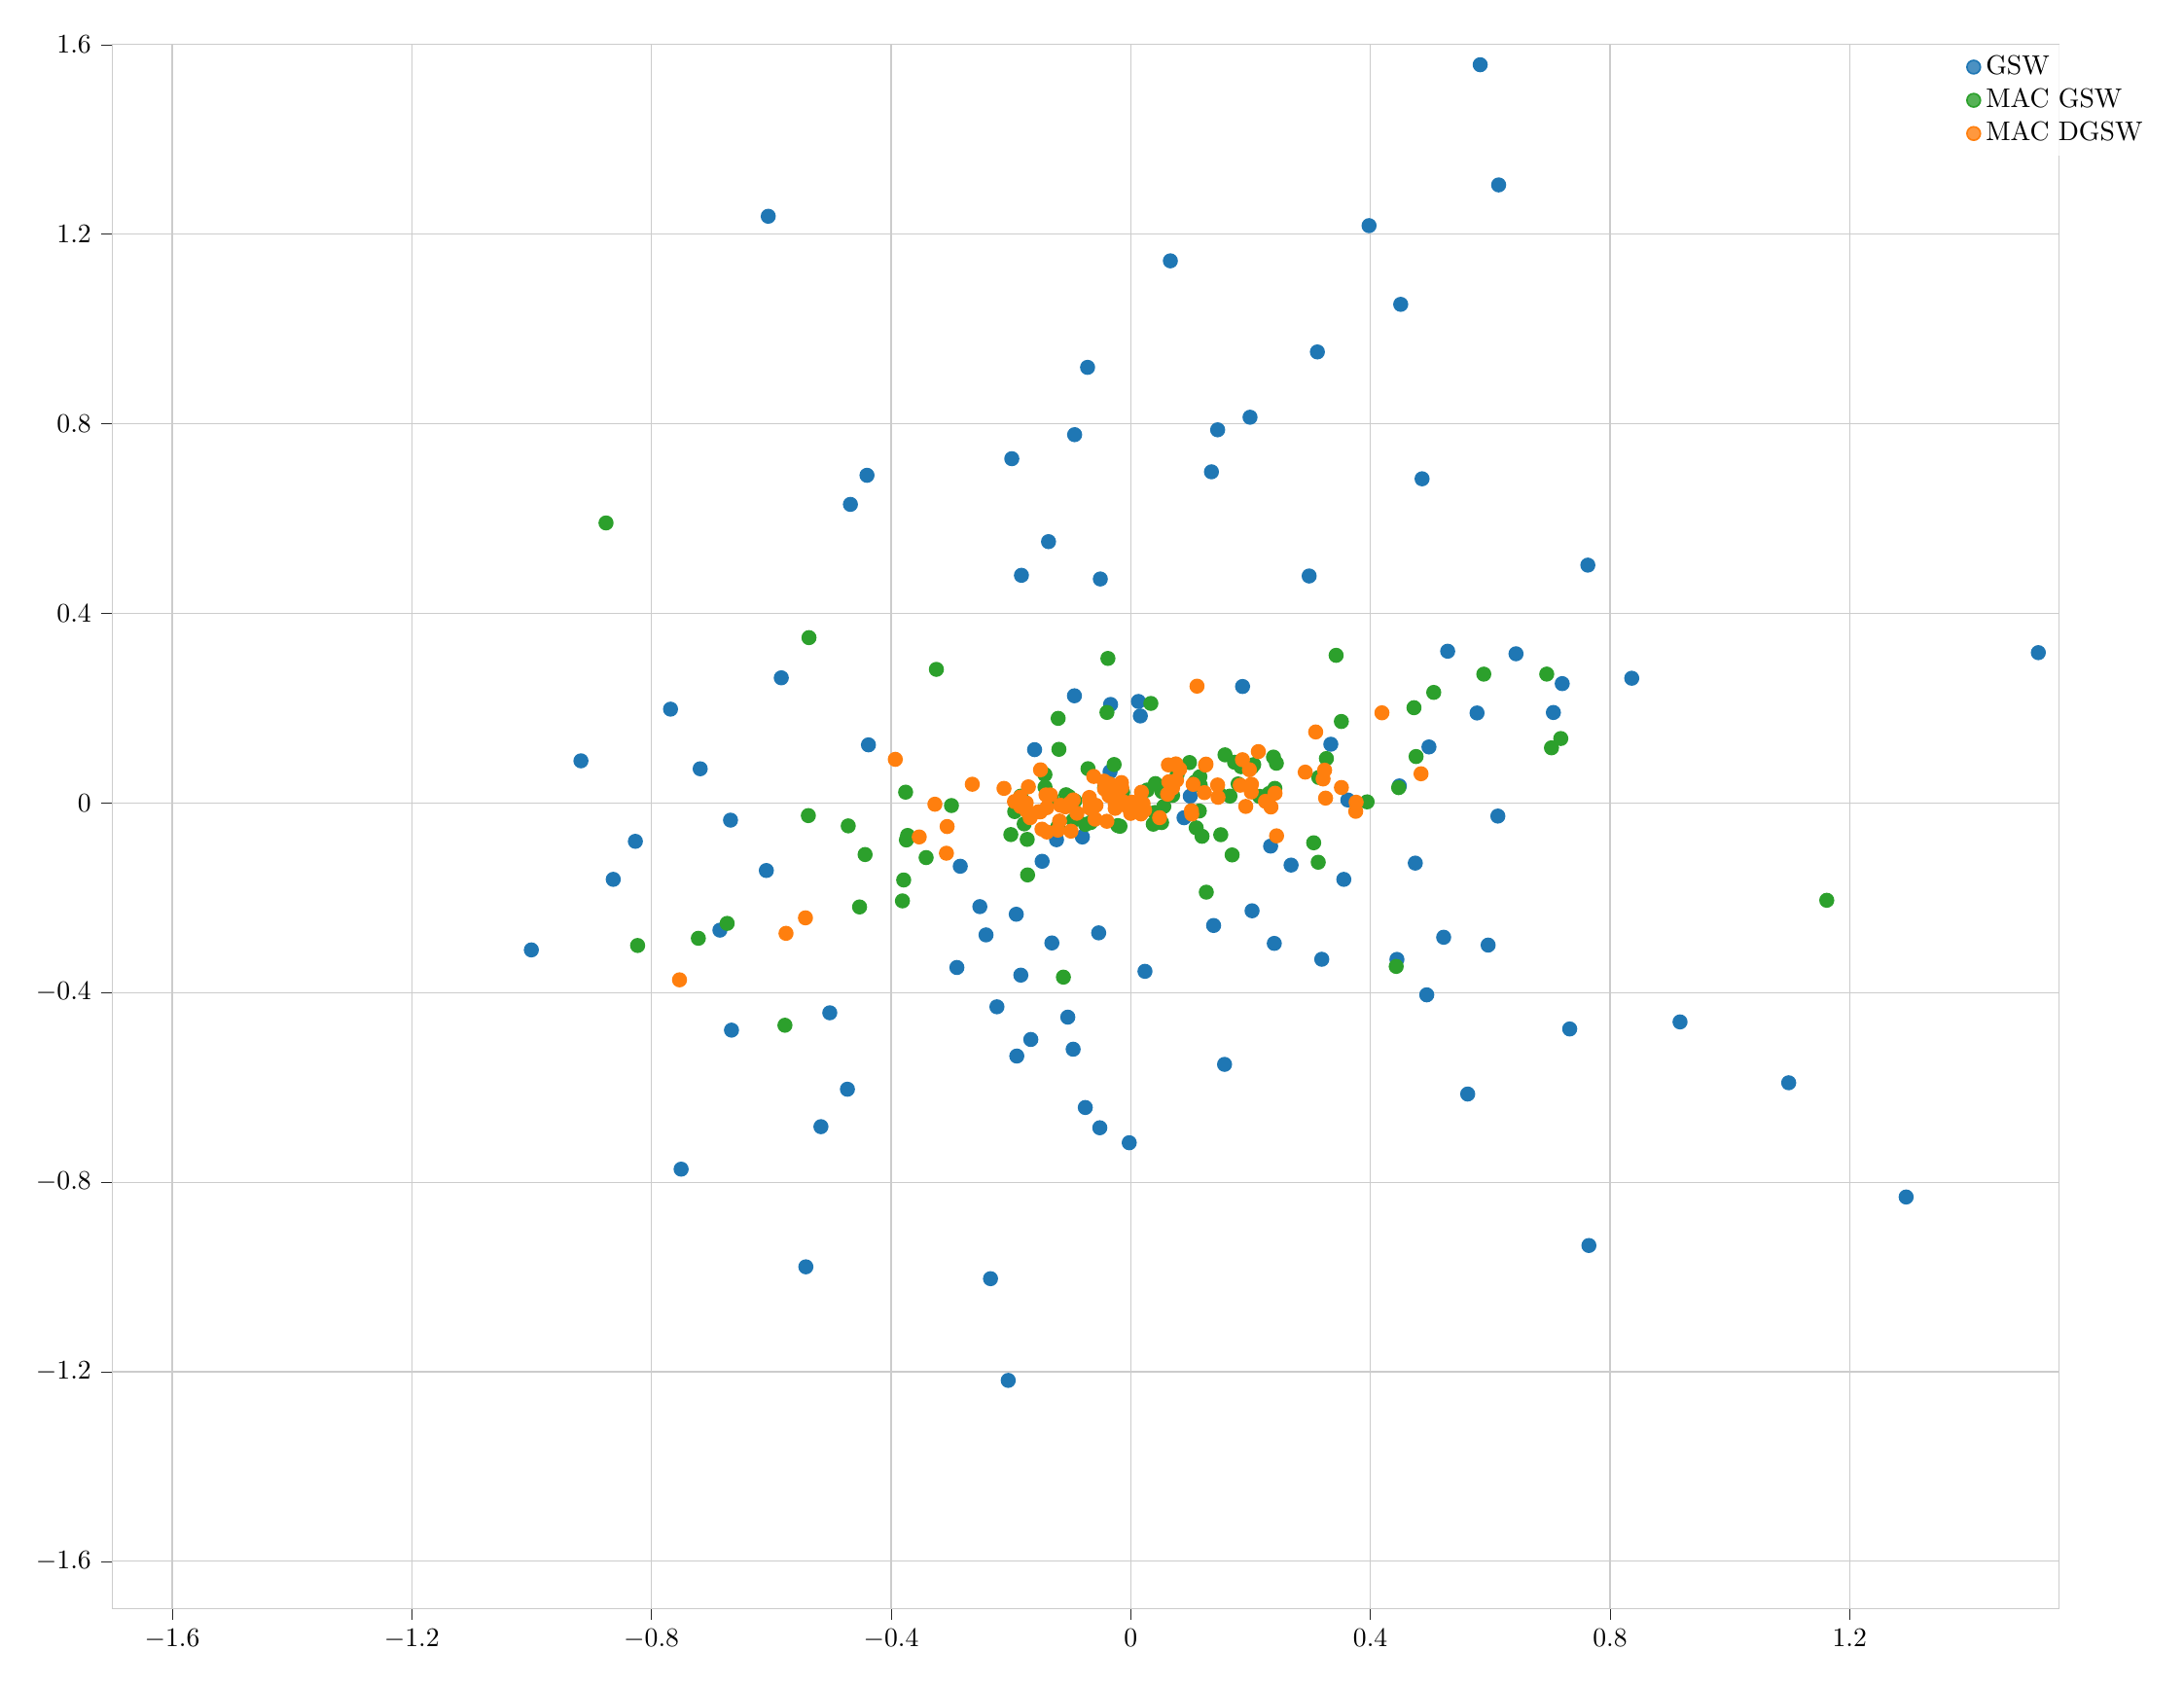
\begin{tikzpicture}

\definecolor{crimson2143940}{RGB}{214,39,40}
\definecolor{darkorange25512714}{RGB}{255,127,14}
\definecolor{darkslategray38}{RGB}{38,38,38}
\definecolor{forestgreen4416044}{RGB}{44,160,44}
\definecolor{lightgray204}{RGB}{204,204,204}
\definecolor{steelblue31119180}{RGB}{31,119,180}

\begin{axis}[
width=27cm,
height=22cm,
axis line style={lightgray204},
legend cell align={left},
legend style={fill opacity=0.8, draw opacity=1, text opacity=1, at={(1.05,1)}, draw=none},
tick align=outside,
tick pos=left,
x grid style={lightgray204},
xmajorgrids,
xmin=-1.7, xmax=1.55,
xtick style={color=darkslategray38},
y grid style={lightgray204},
ymajorgrids,
ymin=-1.7, ymax=1.6,
ytick style={color=darkslategray38},
xtick distance=0.4,
ytick distance=0.4
]
\addplot [semithick, steelblue31119180, mark=*, mark size=2.5, mark options={solid}, only marks]
table {%
-0.234033255900646 -1.00367625019002
-0.502292043921522 -0.442764076039422
0.836281036081821 0.263084517582837
0.138364094176499 -0.258526220858707
0.720248125753671 0.251712751646566
-0.241530179786962 -0.278434880730301
0.0128763064710159 0.214100080883318
-0.204442374925504 -1.21832109870571
-0.608197564356168 -0.14257831092463
-0.0936134180999035 0.776945732312224
-0.00246726984979651 -0.716910161362025
-0.137189984811076 0.551247277714
0.186673795468766 0.2456891065191
0.239637110914271 -0.296353691034541
-0.718623596516722 0.0720362040330895
0.297852963858004 0.478804979559002
-0.750430917872083 -0.772637055145202
0.705507739660454 0.190804869430336
-0.0720022653092329 0.918975982974229
-0.123814909599926 -0.0776276238353677
0.267675758577033 -0.131130422585034
-0.82681530560466 -0.0810171980973629
0.732732709488719 -0.47686808321412
-1.00044502393813 -0.310093229487481
1.29431940394063 -0.831415361862816
0.475008016074183 -0.126943220401025
-0.685714349431893 -0.268399965993668
0.583313456288618 1.55742618164271
0.444369718236827 -0.330112467607311
-0.284503604583435 -0.133606146339581
0.233497309005808 -0.0910962452390574
0.397801468300577 1.2179036546879
-0.050758350904212 0.472484446535623
-0.183434987952764 -0.363305626324016
-0.223302192675715 -0.430129341802673
-0.0534741068054509 -0.274142486626822
0.202541958710536 -0.227564566783066
-0.105038142654043 -0.451936681435429
-0.075848537214351 -0.642583219068994
-0.166753100141519 -0.499067191270763
0.33399504260331 0.123843922697859
-0.0336450301291598 0.207814840092509
0.562472896923732 -0.61414804377299
0.145093422789962 0.787170879612976
0.311567697622262 0.951486970253645
0.91689310603079 -0.462029293363238
-0.517084430567519 -0.683008311536262
0.614135668194764 1.30387815523542
0.529045694787901 0.320050738115971
0.0237974349060753 -0.355277745197299
0.596596302109347 -0.299938385950881
-0.198510437119641 0.726235380064146
-0.0960998131139271 -0.519616751610891
-0.190166247273823 -0.534026535906529
0.764767145434663 -0.933706788175571
0.0889753152224092 -0.0312077873034743
0.36244679028543 0.00624452160930389
0.6128168972278 -0.0277600949820586
-0.191027474026181 -0.234864632153135
0.0160484773037026 0.183466188993843
0.643101908110998 0.314664610624357
-0.440199665544361 0.691239049729156
0.522357308286315 -0.283420746405377
-0.667982451276813 -0.0363005619357031
-0.542228100645402 -0.978698636278002
0.318913269028745 -0.32981670044333
-0.917661964431249 0.0888366355272649
0.0661526864113611 1.14369098033805
0.448420206334977 0.0358587750821122
0.355680921983809 -0.161284019897439
-0.0344789102830596 0.0657710630078346
-0.437768711248302 0.122519762174017
-0.147878149578096 -0.123084827352889
-0.160442437453102 0.112441327899687
-0.467873969950387 0.629851378183047
-0.605004790094052 1.23773238318976
1.09826526258572 -0.590391841218628
0.486323437231879 0.683842148301535
0.49781344085074 0.118138783209857
0.199162579616324 0.813746699815786
0.0994037835743394 0.0143177621005774
0.763008865294524 0.501698765423466
-0.182408913052498 0.480233554589529
-0.472858997530384 -0.60399450758573
-0.290131704232166 -0.347211137555826
0.49412088197899 -0.404874307135683
0.450657852913912 1.05187172477543
-0.0806898339621819 -0.071868882406181
-0.583278838671477 0.263942259852952
0.578072152084348 0.189771221245725
-0.251844989661519 -0.218792848593097
-0.863744368192662 -0.161256459107712
-0.131614768114232 -0.295411293815551
-0.0939281839109833 0.226040429880138
0.156641803715926 -0.551550561227323
-0.666352427418555 -0.479376836175968
-0.768137612744406 0.197861184421593
1.51494426762626 0.317066425699446
0.134735826160048 0.698549161623672
-0.0515880740525029 -0.685313172995431
};
\addlegendentry{GSW}

%\addplot [semithick, darkorange25512714, mark=*, mark size=2, mark options={solid}, only marks]
%table {%
%-0.467038638468901 0.163351498862461
%-0.101919239185745 0.628473700900072
%0.0801924579100065 -0.178704025732937
%0.753187462269824 0.130064491469967
%0.374706860893716 -0.000387992592425224
%-0.665370057589865 0.0977067973338231
%0.652053081628812 0.292598376670511
%0.0148374262245012 0.378243944044846
%0.224735447322395 0.33277893100804
%0.339695432014035 0.220293114276441
%0.694717804129718 -0.484730614404811
%-0.0447768761318819 0.180189466069606
%-0.367025401708594 1.0687999144798
%-0.164054684475613 -0.458662907503445
%0.130221881285737 -0.524035663610767
%0.139814781734605 -0.543560270488167
%-0.962600570869716 -0.405288180125603
%0.973488043120976 -0.856935717130698
%-0.440666815972203 0.280433637963377
%-0.279543693416206 0.647478605973526
%-0.129562555220653 0.0588498091628559
%-0.050620670577852 -0.283010632321553
%0.312804647257637 0.542420767552628
%0.172901039220575 0.308096072147623
%-0.0295902410676738 0.189467024788717
%0.214739519903408 -0.244751086807525
%-0.52024362531045 0.20751662277544
%0.575134510698105 0.192216465590657
%0.150715414211444 -0.711243051143785
%0.765226857889441 0.435857119223086
%-0.227930477381331 1.30418491509201
%-1.34581232354493 0.534977988459928
%0.541398295437146 -0.689140693488258
%0.158009163661221 -0.575798723396934
%-0.110283969633127 -0.737828205205298
%0.294004072225423 0.0636371267252119
%-0.324449474089598 -0.342572150292722
%-0.151939677302189 -0.677225952907154
%0.289978280355074 -1.67142044822281
%0.560658602768102 -0.0849140658534184
%-0.107280888026982 1.15769703648838
%-0.314819239788976 -0.34650834432936
%-1.38391301064195 0.541308226480151
%-0.403737434798016 0.0127302300870335
%-0.217189852665226 -1.26494628164814
%-0.684202923195837 -0.100376911016385
%0.364510233051626 -0.236511476043339
%0.236083118717556 -0.128124242586085
%0.799712056114389 -0.383150421703668
%-0.748713019192892 0.408961673118363
%-0.202722631903016 0.246254463190886
%-0.514198194867251 0.297689359483197
%0.197146403905739 -0.888888552284097
%-0.106590823137342 -0.836970181275125
%0.351658978089219 0.150545401821191
%-0.360664616958125 0.00728441090099902
%-0.772311745710641 -0.748031877030754
%0.803979268759866 -0.532275932049867
%0.404127469582868 0.52052282583965
%0.571727720359632 -0.4122869845535
%-0.49656713035119 0.254312679410066
%-0.473848057608177 -0.462853635482663
%-0.21735193858735 0.160209512945719
%0.348912052619848 -0.0532043387527634
%0.448122238410888 0.0167747642584531
%0.608428829334961 -0.266423999545314
%-0.377289541115829 0.74624134034711
%-0.29943763862136 0.479255261575632
%-1.0799508143577 -0.415839799032266
%-0.0396261025999249 0.231840931307818
%0.262938386809242 0.926279166548501
%-0.422619589658966 0.322946363715624
%-0.233890094862289 0.857701338268492
%-0.260559723624523 -0.343756045118935
%0.0430604414638127 0.754334293069406
%0.0450509234258425 -0.277706956651417
%-0.762037299157703 -1.12434535910064
%-1.70092765813293 -0.260285422727825
%-0.317487208257024 0.0227894113547166
%-0.0958234377251024 0.264701612226168
%-0.323950877294993 -1.18760723318645
%-0.384929040090102 0.309697957903963
%-1.37214395773189 -0.659793972870984
%0.305179407081578 0.588452100742887
%-0.317721638810046 0.228557811586253
%-0.206700043131411 -0.000313817836921138
%-0.532578958505892 0.824388445427596
%-0.132099433765255 -0.83908557519675
%0.790673729882814 0.45270776933461
%0.202017121371984 0.296403517972251
%0.449300888087678 0.053334512732316
%-0.50538117909258 -0.428574039500352
%0.260125371639742 -0.143484256775755
%-0.156476759617417 0.613082101679903
%-1.04544227920129 -0.0632185651588164
%-0.53258455101681 -0.529992899179842
%0.544601773249693 0.241818954253737
%-1.26173673902597 0.205213988866057
%0.192660671855517 0.606290544884742
%0.682584665856881 0.379837987206885
%};
%\addlegendentry{DGSW}
\addplot [semithick, forestgreen4416044, mark=*, mark size=2.5, mark options={solid}, only marks]
table {%
-0.452588602774574 -0.219457519460316
0.476345859537541 0.0978953427767095
-0.172134036025111 -0.151866179644672
-0.0396657886434861 0.190964636126735
0.472817157668971 0.200893147113116
-0.374457774017679 -0.078149422136211
1.16182540485516 -0.20537819098432
-0.0755124028422982 -0.0453587423594553
-0.021250694186526 0.00591169842617756
0.114498859647634 -0.0169505176397957
-0.0276938123583239 0.0810148496112875
0.14969375396652 0.0169376407427895
0.447221674723109 0.0322961476899399
-0.0179316749888104 -0.0492118898425012
-0.200126112195661 -0.0667606289997217
0.15737935214187 0.101437267783666
0.052145845767631 0.0239964360020453
0.126148688291824 -0.188221812062247
0.305412180003018 -0.0840760930397906
-0.721666726034963 -0.285558749136333
-0.172747480854279 -0.0769119456002741
-0.143027073778956 0.0331215668832454
-0.0215992998139061 -0.0477537566915334
0.694392524590123 0.2717972827469
0.20213846865895 0.0756031364328507
0.0552508046433218 -0.00729542986950665
-0.121086237646942 0.178405263015607
0.179342618577572 0.0401050106372966
-0.381015784562271 -0.206682534674106
-0.103020330735049 0.0133818008515392
0.109280628699765 -0.0524947157735565
-0.0436045309481592 0.0319116428663881
0.717826271361302 0.135909663686394
0.702327410990699 0.116280740358789
-0.18357262441467 0.0143560529807855
-0.132321586741959 0.0095982333732853
0.342869252902813 0.311414816003961
0.238284928024251 0.0967131970978064
0.243133392053099 0.0837668590903854
0.184172676340713 0.0765114855097812
0.589323808064775 0.271711416388367
-0.112375218147719 -0.367555419475738
0.077640797486753 0.0609039768626861
-0.673605737892968 -0.254118964628534
-0.119857788044729 0.113067630764945
0.21492665999262 0.0139238402471929
0.240625414196534 0.0307654421395966
0.0403768821095021 -0.0201857966203044
0.173340383895519 0.0858623207290259
0.0980978619403807 0.0852205325145094
0.0101882587167542 -0.00782530215795912
-0.299234588631573 -0.00552398746593336
0.0669749235920836 0.0192430455417744
-0.0670285920129388 -0.041420968277452
-0.341481794137533 -0.11529622529259
-0.378953310834446 -0.162571322653048
0.351603923219323 0.171866440219441
0.115407641915677 0.0552102864977269
0.443123446412395 -0.344928866188997
-0.875785822139023 0.590704877578923
-0.537006404845616 0.348737396631864
0.0411969754590678 0.0407924355875438
0.0698136672868535 0.0160203358858849
-0.375718820001009 0.0227433413507611
-0.823046106197783 -0.300789847174211
-0.143204802744239 0.059737010817174
-0.0899831145902293 -0.0338601753190018
0.165671606473188 0.0144445418355706
-0.0134674860633244 0.0225288219436536
0.20531471583818 0.0808763140579259
0.107472390832947 0.0441193615889207
-0.577153734170454 -0.469032336795373
0.116092580470093 0.037343792022727
-0.471492130020215 -0.0484442264634512
-0.177795342486552 -0.0442462195404794
0.169240160411651 -0.109714681439213
0.0515366746343972 -0.0414838042054453
-0.0712346980302463 0.0722493499102312
0.119034560622277 -0.0703488328239812
-0.0380451427656536 0.304860082254377
0.505770524002574 0.233144975579216
0.0336006398843489 0.209967990026856
-0.372424997164652 -0.0686215382058942
-0.0932944987979305 0.00438616078851911
0.0376116654480543 -0.0448399608999658
-0.0960110854805889 -0.0367298794311169
-0.193660326174418 -0.0182453511125268
-0.443371646852136 -0.108842415006626
-0.538060705063321 -0.0267198262646902
0.326640489319838 0.0936577822292611
-0.12155069079146 -0.0502962347868531
0.23082245011828 0.0198765378934497
0.312980912115538 -0.125105611280891
0.394565201840874 0.00227558535755873
-0.107965869020627 0.0172665394403077
0.150286699401742 -0.0670258963231307
-0.324379012168804 0.281801719790688
0.31386641253924 0.0537285859365982
0.0275597383415886 0.0272938668757595
-0.0113449086065469 0.00309961602242942
};
\addlegendentry{MAC GSW}
\addplot [semithick,darkorange25512714, mark=*, mark size=2.5, mark options={solid}, only marks]
table {%
-0.0259290885910473 -0.0114954142409386
0.101271357186816 -0.0163255681630171
0.321070395965924 0.0505440489372534
-0.140059957970794 -0.0100182357410043
-0.173724007349841 -0.01659947126851
0.0178994088758675 0.0226494928837153
0.323589723140104 0.0690639344764825
-0.121653065697466 -0.0573876017212023
0.145758540288976 0.0118743706290425
-0.542913255689161 -0.242433510301094
-0.044519808936015 0.0460174908431399
-0.264423422334665 0.0394456110189793
-0.0996860933075897 -0.0595836391533731
-0.194042406891768 0.00282331831890043
-0.150840159398639 -0.0188512231886781
-0.00504781942925503 -0.00803396232462489
0.201222555600259 0.0231446372915483
-0.575363458117484 -0.275118126046534
0.0816661332083763 0.0713452730752241
-0.170814674940205 0.0339744541043389
-0.306425737204616 -0.0497798024435666
-5.92512676844681e-05 -0.0220339074893874
0.351673869362231 0.0325244217968411
-0.0686640112706358 0.00434780414224539
-0.753123446011497 -0.373216500117259
0.11068452904831 0.246368423949788
0.30874631939003 0.149719714211031
0.0163944217345366 -0.0171918133635158
0.145029742213559 0.0378682029138547
-0.0617587675667626 0.0558898803027492
-0.0137097546900626 0.0036246259937967
0.484585317000591 0.061541622566999
-0.16779531256401 -0.0311279341558582
0.0482001087126991 -0.0311249338900673
0.419317515267764 0.190112550140946
-0.117238233442065 -0.00487364399628099
0.201547530343832 0.0393796467379078
-0.014863319531324 0.0322127543024764
-0.139901828639746 -0.0612694566959325
0.0231189245805801 -0.0151807269599253
0.125708258622434 0.0818705515724565
-0.0188690361759881 -0.00287549992783936
0.0667146603981974 0.0397880503781795
0.0615173906748752 0.0184856817435434
-0.108933327414126 -0.00824240251889535
0.186514313850463 0.0911723672182451
-0.0154881063237819 0.0429026867853062
-0.174444152662411 9.53316863138709e-05
0.0206273810170188 -0.00139224782225739
0.291282613640035 0.0650094803971125
-0.0258917298780877 -0.00242251785998976
0.0764493482773496 0.0477516389796031
0.0171140202697303 -0.023220488211578
0.240881617500477 0.0204892508265295
-0.150571506393192 0.0698832608038778
-0.0624598421215201 -0.00806022534590595
0.00127917869456717 -0.00259887136416576
-0.0398215158445897 -0.0386487749146161
0.0698264882035515 0.0316239716613911
0.213041256529099 0.108370926590979
0.192018622007245 -0.00735777965802381
0.2249343092522 0.00336225175985977
-0.0897570130146476 -0.0217210910215295
-0.0579589471424498 -0.00510737680028422
-0.154071596242187 -0.0186809814167616
0.123019176489109 0.021721573101557
0.101871203764898 -0.0235054359763387
-0.0362437434355024 0.0154239337308216
-0.0683513562768572 -0.0107507334284637
0.0636355550669276 0.0446815130378973
0.182728075687153 0.0373908375410564
-0.30760575387384 -0.106099048416679
-0.141460295122937 0.0169513047282338
-0.101669373316617 -0.000887061823747592
-0.059534758047632 -0.0342415916737528
-0.0690802470571918 0.011507375166087
-0.32685351536921 -0.00272643822790314
-0.148200441044484 -0.0553101829727871
-0.211529856327678 0.0306700586475537
-0.118787143598226 -0.0380351474304789
0.104195933095623 0.0392436008679081
-0.0317941510545268 0.0145798532192029
0.12478346412891 0.0798784515913161
-0.352992770510152 -0.0717584977079477
-0.034834721109417 0.0398992559646995
0.375539437802883 -0.0177353861727488
0.234084158594843 -0.00856200937626878
-0.184391506391315 0.0122843241158181
0.243452458208886 -0.0694527300099564
0.198123289662619 0.0700542613139712
0.0628562363675892 0.0802458095633186
0.0754791742508432 0.082331090375258
0.376266722862813 0.0014674573418863
-0.134075805746529 0.0169151489769553
-0.0958566581654372 0.00638274823300239
0.325233699994208 0.0101685007957334
0.00189541438991614 0.00157168089287324
-0.39294081003627 0.0919894543494698
-0.183729016246042 -0.00746808728097409
-0.0435006189087979 0.029219668306913
};
\addlegendentry{MAC DGSW}
\end{axis}
\end{tikzpicture}\label{max_col_comp}
\vspace{-1ex}
\end{tikzfigure}}
%100 points for each variant on the graph.

\block[bodyinnersep=0.4cm]{Going Further}{
There are various areas where this algorithm could be improved and better understood:
\begin{itemize}
\item The choice of the direction could be changed slightly to adapt it to some problematic inputs that exist for $n>d$. 
\item The pivot choice could be done in many ways to improve some aspects. 
\item The input vectors could be modified to add additional known information or constraints about the assignment.
\item The modification discussed in my thesis, that minimizes balance in a certain way, could certainly be better understood. 
\item The algorithm could be generalized to separate inputs into more than 2 groups in a single run.
\end{itemize}
Additionally, it would also be interesting to explore further the use of the algorithm to solve problems regarding hidden substructures in large sets, such as the planted clique, or the potential usages of a vector balancing algorithm in machine learning.
}

\end{columns}
\end{document}

%Cool todo: remove end in while loop